% Section 4: System Requirements
\section{System Requirements}

This section specifies the system requirements at different levels: domain, product, data, and quality. The requirements have been elicited through the techniques described in Section 3 and are documented using multiple specification techniques to ensure comprehensive coverage and clarity for all stakeholders.

\vspace{0.3cm}

\textbf{Specification Techniques Used:}

The following specification techniques have been employed to document the CookWise system requirements:

\begin{enumerate}
    \item \textbf{Context Diagram} (Section 1.5): Visual representation of the system boundaries and external entities, showing how CookWise interacts with users, stores, and external services.

    \item \textbf{Use Case Diagrams} (Section 4.2): Visual representation of user interactions with the system, showing both the overall system use cases and a detailed view of the core recipe browsing workflow.

    \item \textbf{Feature Requirements} (Textual): Product-level requirements (PR1-PR15) are specified as textual "shall" statements describing specific system capabilities and behaviors.

    \item \textbf{Data Model (Entity-Relationship Diagram)} (Section 4.4): Visual representation of all data entities, their attributes, and relationships using an ERD to ensure database design clarity.

    \item \textbf{Data Dictionary} (Section 4.4): Textual description of all data requirements (DR1-DR4) covering core entities, relationships, data formats, and system configuration.

    \item \textbf{Domain Rules} (Section 4.1): Textual specification of business rules and constraints (DL1-DL6) that define the problem domain and operational boundaries.

    \item \textbf{Quality Requirements Specification} (Section 4.5): Structured specification of non-functional requirements (QR1-QR5) with measurable quality attributes using the QUPER model.
\end{enumerate}

\vspace{0.3cm}

This combination of techniques ensures that requirements are communicated effectively to different stakeholders: visual models for system architects and developers, textual specifications for business stakeholders and testers, and structured quality metrics for project managers and quality assurance teams.

\subsection{Domain Level Requirements}

\noindent\textbf{DL1:} The system's core product and pricing data shall be sourced from grocery store websites through web scraping.

\textbf{DL2:} The system operations shall comply with relevant data protection regulations (e.g., GDPR) regarding user and partner data.

\textbf{DL3:} The system shall ensure all shopping lists contain only items available at a single physical store location (single-store shopping constraint).

\textbf{DL4:} The calculation of a store's total basket price shall include all applicable promotions and discounts for the user.

\textbf{DL5:} The system shall enforce rate limits and operational boundaries for external interfaces (web scraping limited to once daily per retailer, AI API limited to 100 requests per hour per user, geolocation API limited to 50 requests per user per day, and session timeout set to 30 minutes).

\textbf{DL6:} The system shall process domain events triggered by user actions (login, search, filter, select), external service responses (AI recipe generation, geolocation queries, authentication validation), and scheduled operations (daily web scraping at 02:00 local time).

\subsection{Use Case Specification}

The following use case diagrams illustrate the functional interactions between users and the CookWise system. These diagrams complement the product requirements by visualizing the user's journey through the system.

\vspace{0.5cm}

\noindent\textbf{Overall System Use Cases}

Figure \ref{fig:usecase_overall} presents an overview of all primary use cases available to users in the CookWise system. The diagram shows that recipe browsing is dependent on store selection (<<include>> relationship), and shopping list creation follows from recipe browsing. The use cases are ordered from top to bottom following the typical user flow: login, store selection, recipe browsing, and supporting features.

\begin{figure}[H]
    \centering
    \includegraphics[width=0.95\textwidth]{images/usecase_overall.png}
    \caption{Overall System Use Case Diagram for CookWise}
    \label{fig:usecase_overall}
\end{figure}

\noindent\textbf{Detailed Use Case: Browse Recipes from Store Sale Items}

Figure \ref{fig:usecase_browse_detail} provides a detailed view of the core use case "Browse Recipes from Store Sale Items." This use case represents the primary value proposition of CookWise: enabling users to discover recipes based on current sales at their selected grocery store. The diagram shows the main flow (blue) with required steps (<<include>> relationships) and optional extensions (yellow) such as filtering, searching, and viewing details (<<extend>> relationships). The PlantUML source code for both diagrams is provided in Appendix C.

\begin{figure}[H]
    \centering
    \includegraphics[width=0.95\textwidth]{images/usecase_browse_detail.png}
    \caption{Detailed Use Case: Browse Recipes from Store Sale Items}
    \label{fig:usecase_browse_detail}
\end{figure}

\subsection{Functional Product Level Requirements}

\noindent\textbf{PR1:} The system shall authenticate users through external authentication services (e.g., Google/Apple ID).

\textbf{PR2:} The system shall invoke the AI Recipe Generation API with currently discounted ingredients, user dietary restrictions, and cuisine preferences to generate recipe suggestions.

\textbf{PR2.1:} The system shall display the top 5 AI-generated recipes ranked by cost savings.

\textbf{PR3:} The system shall filter recipe search results based on cuisine, dietary restrictions (e.g., vegan, gluten free), budget, cooking time, difficulty level, and user ratings.

\textbf{PR4:} The system shall automatically generate a consolidated shopping list when the user selects one or more recipes, aggregating ingredient quantities for duplicates and applying current sale prices where available.

\textbf{PR5:} The system shall record individual user ratings (1-5 scale) and text feedback submitted by users for recipes.

\textbf{PR6:} The system shall store recipes generated by AI and their details (e.g., id, ingredients, instructions, rating).

\textbf{PR7:} The system shall display recipe details including ingredients, cooking time, difficulty level, step by step cooking instructions, and nutritional data.

\textbf{PR8:} The system shall display store price comparisons and distances from user location for each store carrying the shopping list items.

\textbf{PR9:} The system shall display total savings amount and itemized price differences between regular and sale prices.

\textbf{PR10:} The system shall display recipes containing ingredients specified in the user's search query.

\textbf{PR11:} The system shall display all ingredients needed for selected recipes, highlighting which ingredients are currently on sale and listing sale items first in the display order.

\textbf{PR12:} The system shall gather and update product data (product name, regular price, sale price, discount percentage, sale validity dates, and product category) from grocery store websites through web scraping once per day at 02:00 local time (scheduled during low-traffic hours to minimize server load on retailer websites and ensure stores have updated their daily promotions).

\textbf{PR13:} The system shall store user preferences for ingredients and recipes.

\textbf{PR14:} The system shall provide store location information with "Get Directions" links that redirect users to their preferred external mapping application (Google Maps, Apple Maps, etc.) with the selected store address pre-populated.

\textbf{PR15:} The system shall calculate and display the average rating (aggregated from all user ratings per PR5) for each recipe, showing both the numerical average and the total number of ratings.

\subsection{Data Requirements}

\textbf{Database Model Selection:} The CookWise system will use a **relational database model** (SQL-based). This decision is based on the structured nature of the data, the need for complex relationships between entities (recipes, ingredients, stores, users), and the requirement for transactional integrity when managing shopping lists. A relational model ensures data consistency, supports complex joins for recipe recommendations, and provides ACID properties essential for data management operations.

\vspace{0.3cm}

\noindent\textbf{DR1: Core Entity Data Models:} The system shall implement the following core entities as specified in the Entity-Relationship Diagram (Figure \ref{fig:erd_diagram}):

\begin{itemize}
    \item \textbf{User:} User ID, Email, Authentication Provider (Google/Apple), Geographic Location (Latitude and Longitude), and Dietary Restrictions
    \item \textbf{Recipe:} Recipe ID, Recipe Name, Cuisine Type, Cooking Time, Difficulty Level, Number of Servings, Step-by-step Instructions, and Image URL
    \item \textbf{Ingredient:} Ingredient ID, Ingredient Name, and Category
    \item \textbf{Rating:} Rating ID, User ID reference, Recipe ID reference, and Rating Score (1-5 scale)
    \item \textbf{Store:} Store ID, Store Name, and Geographic Coordinates (Latitude and Longitude)
    \item \textbf{Sale Item:} Sale ID, Store ID reference, Ingredient ID reference, Sale Price, and validity period (Valid From date and Valid To date) to track promotional pricing offered by grocery stores on specific ingredients
\end{itemize}

\vspace{0.3cm}

\textbf{DR2: Relationship and Associative Entity Data Models:} The system shall implement the following relationship tables to connect core entities:

\begin{itemize}
    \item \textbf{Recipe-Ingredient:} Recipe ID reference, Ingredient ID reference, Quantity, and Unit to specify exactly how much of each ingredient is needed for a recipe
    \item \textbf{Shopping List:} List ID, User ID reference, Store ID reference to link each shopping list to a specific user and their chosen store, and Total Price to track the aggregate cost of all items
    \item \textbf{Shopping List Item:} List ID reference, Ingredient ID reference, Quantity to specify the amount needed, and Sale ID reference to track which specific sale promotion is applied to each item for accurate savings calculation
\end{itemize}

\vspace{0.3cm}

\textbf{DR3: Data Interchange Formats and Communication Protocols:} The system shall support the following data formats for external communication:

\begin{itemize}
    \item \textbf{API Communications:} JSON format for all API communications with external services (AI recipe generation, geolocation, authentication)
    \item \textbf{Data Export:} CSV and JSON formats for user data export functionality
    \item \textbf{Web Scraping:} Structured HTML parsing for data extraction from grocery store websites
    \item \textbf{Encoding:} UTF-8 encoding for all API requests and responses following RESTful conventions
\end{itemize}

\vspace{0.3cm}

\textbf{DR4: System States and Initial Data Configuration:} The system shall maintain the following operational states and be initialized with seed data:

\begin{itemize}
    \item \textbf{User Session States:} Anonymous, Authenticated, Active, Expired
    \item \textbf{System Operational States:} Idle, Scraping Data, Processing Requests, Maintenance Mode, Error State
    \item \textbf{Recipe Generation States:} Pending, In Progress, Completed, Failed
    \item \textbf{Shopping List States:} Draft, Finalized, Archived
    \item \textbf{Initial Seed Data:} Minimum of 100 recipes across various cuisines, complete store information for major ICA, Willys, and Coop locations in target regions, comprehensive ingredient database with at least 500 common ingredients, and default user preferences (Swedish language, metric measurements, no dietary restrictions, 30-minute default cooking time filter)
\end{itemize}

\noindent\textbf{Entity Relation Diagram}

The Entity Relation Diagram (ERD) below illustrates the data model for the CookWise system. The diagram shows the relationships between all entities and their attributes. The system uses a relational database model to ensure data integrity and support complex queries required for recipe recommendations and shopping list optimization.

\vspace{0.5cm}

\textbf{Key Entities and Relationships:}

The data model is organized around four core workflows:

\textbf{1. Recipe Discovery and Rating:} Users can browse recipes, view their ingredients through the RECIPE\_INGREDIENT relationship, and provide ratings. This enables the system to recommend popular recipes and track user preferences.

\textbf{2. Sale and Promotion Management:} Stores offer sale items on specific ingredients, tracked through the SALE\_ITEM entity. This connection between stores and ingredients enables the core functionality of suggesting recipes based on current promotions, with each sale item having a sale price and validity period.

\textbf{3. Ingredient Management:} The INGREDIENT entity serves as the central hub connecting recipes, shopping lists, and sales. Each ingredient has a name and category, enabling efficient search and organization across all system features.

\textbf{4. Shopping List Management:} Users create shopping lists that contain specific ingredients with quantities. Each shopping list is linked to a single store and tracks the total price. The SHOPPING\_LIST\_ITEM entity references which specific sales are applied to calculate accurate savings.

The model ensures single-store shopping (as per DL3) by linking each shopping list to one store through the STORE entity, while enabling price optimization by tracking which sale items are applied to each shopping list item.

\begin{figure}[H]
    \centering
    \includegraphics[width=1.0\textwidth]{images/erd_diagram.png}
    \caption{Entity Relation Diagram for CookWise System}
    \label{fig:erd_diagram}
\end{figure}

The complete PlantUML source code for this diagram is provided in Appendix B.

\vspace{0.5cm}

\noindent\textbf{Virtual Windows}

Virtual windows illustrate how data will be presented to users through simplified screen mockups with realistic data. These windows demonstrate the key data flows and user interactions without detailed UI elements like buttons or menus.

\vspace{0.3cm}

\textbf{Virtual Window 1: Recipe Detail View}

This window shows how recipe data is presented to users, including ingredients with sale indicators, cooking details, and pricing information.

\begin{table}[H]
\centering
\fbox{\begin{tabular}{p{13cm}}
\multicolumn{1}{c}{\textbf{\large Swedish Meatballs with Cream Sauce}} \\[0.3cm]
\hline
\\[-0.2cm]
\textbf{Cuisine:} Swedish \quad \textbf{Cooking Time:} 35 minutes \quad \textbf{Difficulty:} Medium \\
\textbf{Servings:} 4 people \quad \textbf{Average Rating:} 4.5/5 (24 ratings) \\[0.2cm]
\hline
\\[-0.2cm]
\textbf{Ingredients:} \\[0.1cm]
\quad $\bullet$ Ground beef, 500g \quad \textcolor{red}{\textbf{ON SALE}} \quad Regular: 89 kr $\rightarrow$ Sale: 59 kr \\
\quad $\bullet$ Breadcrumbs, 100g \\
\quad $\bullet$ Onion, 1 medium \\
\quad $\bullet$ Heavy cream, 200ml \quad \textcolor{red}{\textbf{ON SALE}} \quad Regular: 28 kr $\rightarrow$ Sale: 19 kr \\
\quad $\bullet$ Butter, 50g \\
\quad $\bullet$ Beef broth, 250ml \quad \textcolor{red}{\textbf{ON SALE}} \quad Regular: 15 kr $\rightarrow$ Sale: 11 kr \\
\quad $\bullet$ Salt and pepper to taste \\[0.2cm]
\hline
\\[-0.2cm]
\textbf{Instructions:} \\[0.1cm]
1. Mix ground beef, breadcrumbs, chopped onion, salt and pepper. Form into small meatballs. \\
2. Fry meatballs in butter until golden brown on all sides (about 10 minutes). \\
3. Remove meatballs, add cream and beef broth to pan. Simmer for 5 minutes. \\
4. Return meatballs to sauce and cook for additional 10 minutes. \\[0.2cm]
\hline
\\[-0.2cm]
\textbf{Your Savings:} \\
\quad Regular Total: 132 kr \quad \textbf{Sale Total: 89 kr} \quad \textcolor{green}{\textbf{You save: 43 kr (33\%)}} \\[0.1cm]
\end{tabular}}
\caption{Virtual Window 1: Recipe Detail with Sale-Based Ingredients}
\label{tab:vw1_recipe}
\end{table}

\vspace{0.3cm}

\textbf{Virtual Window 2: Shopping List View}

This window demonstrates how the shopping list aggregates ingredients from multiple selected recipes, applies sale prices, and calculates total savings.

\begin{table}[H]
\centering
\fbox{\begin{tabular}{p{13cm}}
\multicolumn{1}{c}{\textbf{\large My Shopping List}} \\[0.2cm]
\multicolumn{1}{l}{\textbf{Selected Store:} ICA Maxi Karlskrona} \\
\multicolumn{1}{l}{\textbf{Recipes:} Swedish Meatballs (4 servings), Pasta Carbonara (4 servings)} \\[0.2cm]
\hline
\\[-0.2cm]
\textbf{Dairy \& Eggs} \\
\quad $\bullet$ Heavy cream, 400ml \quad \textcolor{red}{\textbf{SALE}} \quad 38 kr \quad (Regular: 56 kr) \\
\quad $\bullet$ Parmesan cheese, 100g \quad 45 kr \\
\quad $\bullet$ Eggs, 6 pieces \quad \textcolor{red}{\textbf{SALE}} \quad 25 kr \quad (Regular: 32 kr) \\
\quad $\bullet$ Butter, 100g \quad 18 kr \\[0.2cm]
\textbf{Meat \& Seafood} \\
\quad $\bullet$ Ground beef, 500g \quad \textcolor{red}{\textbf{SALE}} \quad 59 kr \quad (Regular: 89 kr) \\
\quad $\bullet$ Bacon, 200g \quad \textcolor{red}{\textbf{SALE}} \quad 35 kr \quad (Regular: 48 kr) \\[0.2cm]
\textbf{Pantry \& Dry Goods} \\
\quad $\bullet$ Spaghetti pasta, 500g \quad 15 kr \\
\quad $\bullet$ Breadcrumbs, 100g \quad 12 kr \\
\quad $\bullet$ Beef broth, 250ml \quad \textcolor{red}{\textbf{SALE}} \quad 11 kr \quad (Regular: 15 kr) \\[0.2cm]
\textbf{Fresh Produce} \\
\quad $\bullet$ Onion, 2 medium \quad 8 kr \\
\quad $\bullet$ Garlic, 3 cloves \quad 5 kr \\[0.2cm]
\hline
\\[-0.2cm]
\textbf{Price Summary:} \\
\quad Regular Total Price: 338 kr \\
\quad \textbf{Your Total with Sales: 271 kr} \\
\quad \textcolor{green}{\textbf{Total Savings: 67 kr (20\%)}} \\
\quad Number of items on sale: 5 out of 11 \\[0.1cm]
\end{tabular}}
\caption{Virtual Window 2: Shopping List with Aggregated Ingredients and Pricing}
\label{tab:vw2_shoppinglist}
\end{table}

\vspace{0.3cm}

\textbf{Virtual Window 3: Store Price Comparison View}

This window shows how the system compares total shopping list prices across different stores, helping users make informed decisions about where to shop.

\begin{table}[H]
\centering
\fbox{\begin{tabular}{p{13cm}}
\multicolumn{1}{c}{\textbf{\large Compare Stores for Your Shopping List}} \\[0.2cm]
\multicolumn{1}{l}{\textbf{Shopping List:} Swedish Meatballs + Pasta Carbonara (11 items)} \\
\multicolumn{1}{l}{\textbf{Your Location:} Karlskrona City Center} \\[0.2cm]
\hline
\\[-0.2cm]
\textbf{Store 1: ICA Maxi Karlskrona} \quad \textcolor{green}{\textbf{BEST PRICE}} \\
\quad Distance from you: 2.3 km (7 min drive) \\
\quad Items on sale: 5 out of 11 \\
\quad Regular total: 338 kr \\
\quad \textbf{Your total with sales: 271 kr} \\
\quad \textcolor{green}{\textbf{You save: 67 kr (20\%)}} \\[0.3cm]

\textbf{Store 2: Willys Karlskrona} \\
\quad Distance from you: 1.8 km (6 min drive) \\
\quad Items on sale: 3 out of 11 \\
\quad Regular total: 325 kr \\
\quad \textbf{Your total with sales: 289 kr} \\
\quad You save: 36 kr (11\%) \\[0.3cm]

\textbf{Store 3: Coop Karlskrona} \\
\quad Distance from you: 3.1 km (9 min drive) \\
\quad Items on sale: 4 out of 11 \\
\quad Regular total: 342 kr \\
\quad \textbf{Your total with sales: 298 kr} \\
\quad You save: 44 kr (13\%) \\[0.2cm]
\hline
\\[-0.2cm]
\textbf{Recommendation:} \\
\quad ICA Maxi offers the best price for your shopping list, saving you an additional \\
\quad 18 kr compared to Willys and 27 kr compared to Coop. \\[0.1cm]
\end{tabular}}
\caption{Virtual Window 3: Store Price Comparison and Recommendation}
\label{tab:vw3_comparison}
\end{table}

\vspace{0.3cm}

These virtual windows demonstrate the core data presentation requirements for CookWise:

\begin{itemize}
    \item \textbf{Recipe data integration:} Combining recipe details (DR1), ingredient information (DR1, DR2), and sale price data (DR1) to highlight cost-saving opportunities for users
    \item \textbf{Shopping list aggregation:} Consolidating ingredients from multiple recipes (DR2) with accurate quantity calculations and price totals including sale discounts
    \item \textbf{Multi-store comparison:} Presenting store information (DR1), location data, and total basket prices across different retailers to support informed shopping decisions
    \item \textbf{Visual sale indicators:} Clear marking of discounted items to immediately communicate savings opportunities to users
    \item \textbf{Savings calculations:} Transparent display of regular prices versus sale prices with percentage savings to demonstrate value proposition
\end{itemize}

\subsection{Product Quality Requirements}

This section defines the non-functional characteristics of CookWise through five quality requirements covering accuracy, reliability, performance, usability, and scalability. Each requirement is specified as a measurable "shall" statement with defined validation procedures.

\subsubsection{Quality Requirements Summary}

Table \ref{tab:qr_summary} presents all quality requirements for the CookWise system:

\begin{table}[H]
\centering
\caption{CookWise Quality Requirements Summary}
\label{tab:qr_summary}
\begin{tabular}{|p{1.5cm}|p{3cm}|p{8.5cm}|p{1.5cm}|}
\hline
\textbf{ID} & \textbf{Quality Aspect} & \textbf{Requirement} & \textbf{Target} \\
\hline
QR1 & Accuracy & The system shall achieve at least 95\% accuracy in sale price data, measured as the percentage of sale prices that match actual retailer prices. & 95\% \\
\hline
QR2 & Reliability & The system shall maintain at least 98\% uptime during peak usage hours (17:00-20:00 local time), measured as the percentage of time the application is fully operational and accessible. & 98\% \\
\hline
QR3 & Performance & The system shall generate recipe suggestions within 5 seconds for 95\% of user requests, measured from the time a user submits search criteria to when results are displayed. & 5 sec \\
\hline
QR4 & Usability & The system shall enable new users to complete their first recipe selection within 8 minutes of account creation, measured from login to adding a recipe to their shopping list. & 8 min \\
\hline
QR5 & Scalability & The system shall support at least 300 concurrent users while maintaining acceptable performance (response time under 10 seconds), measured during peak usage hours. & 300 users \\
\hline
\end{tabular}
\end{table}

\vspace{0.3cm}

\textbf{QUPER Analysis Approach:} Two quality requirements (QR1 and QR5) undergo detailed QUPER analysis due to their complexity and cost implications, while QR2, QR3, and QR4 have straightforward targets.

\subsubsection{QR1: Accuracy - Price Data Correctness (QUPER Analysis)}

\textbf{Requirement:} The system shall achieve at least 95\% accuracy in sale price data, measured as the percentage of ingredient sale prices that match actual current sale prices published by retailers.

\vspace{0.2cm}

\textbf{Rationale:} Accuracy is critical for user trust and cost savings. Different accuracy levels require different technical approaches, making QUPER analysis valuable for understanding cost benefit tradeoffs.

\begin{table}[H]
\centering
\begin{tabular}{|p{14cm}|}
\hline
\textbf{FEATURE:} Sale Price Information \\
\textbf{ID:} QR1 \\
\textbf{QUALITY REQUIREMENT:} Accuracy of sale prices \\
\hline
\textbf{DEFINITION:} The percentage of ingredient sale prices in the application that match the actual current sale prices published by retailers, measured as (number of correct prices / total number of sale prices) × 100. \\
\hline
\textbf{REFERENCE LEVELS} \\
\textbf{PRODUCT:} eTilbudsavis \textbf{LEVEL:} 95\% accuracy \\
\textbf{PRODUCT:} Price comparison websites \textbf{LEVEL:} 85-90\% accuracy \\
\textbf{PRODUCT:} Current CookWise \textbf{LEVEL:} N/A (new system) \\
\hline
\textbf{QUALITY BREAKPOINTS} \\
\textbf{UTILITY:} 90\% accuracy \textbf{RATIONALE:} Below 90\%, users lose trust in recommendations. One in ten incorrect prices creates too many negative experiences and undermines cost savings value proposition. \\
\textbf{SATURATION:} 100\% accuracy \textbf{RATIONALE:} Perfect accuracy impossible with web scraping due to timing delays, retailer website changes, and regional variations. Diminishing returns beyond 98-99\%. \\
\textbf{DIFFERENTIATION:} 98\% accuracy \textbf{RATIONALE:} Accuracy of 98\%+ establishes application as highly reliable and trustworthy. Can be promoted as "verified sale prices" for strong competitive advantage. \\
\hline
\textbf{COST BARRIERS AND TECHNIQUES} \\
\textbf{Qref:} 92\% accuracy - Basic web scraping with simple validation \\
\textbf{Q1:} 96\% accuracy \textbf{RATIONALE:} Advanced parsing algorithms, automated validation checks, error detection and correction systems. Requires sophisticated data validation logic for multiple retailer formats. Moving beyond 96\% requires switching to or supplementing with API integrations instead of web scraping alone. \\
\textbf{C1:} 2 weeks \\
\textbf{Q2:} 99\% accuracy \textbf{RATIONALE:} Multi-source validation combining web scraping with retailer API access (where available), cross-verification against multiple data points, and machine learning for anomaly detection. Requires partnerships with retailers and sophisticated data reconciliation. \\
\textbf{C2:} 16 weeks \\
\hline
\textbf{TARGETS} \\
\textbf{GOOD:} 95\% accuracy \textbf{RATIONALE:} Reliable enough for confident purchasing decisions, matches best available competitor (eTilbudsavis), achievable with robust web scraping implementation and validation checks. \\
\textbf{STRETCH:} 97\% accuracy \textbf{RATIONALE:} Provides differentiation through advanced web scraping techniques, automated error correction, and multi-source data validation systems. \\
\hline
\textbf{VALIDATION PROCEDURE} \\
Accuracy validated through weekly manual verification tests. Random sample of 100 sale items selected from database and manually checked against current retailer websites and physical store flyers. Percentage of matching prices calculated. Additionally, users can report incorrect prices through application for ongoing accuracy monitoring. \\
\hline
\end{tabular}
\caption{QR1: Accuracy Quality Requirement with QUPER Analysis}
\label{tab:qr1}
\end{table}

\begin{figure}[H]
    \centering
    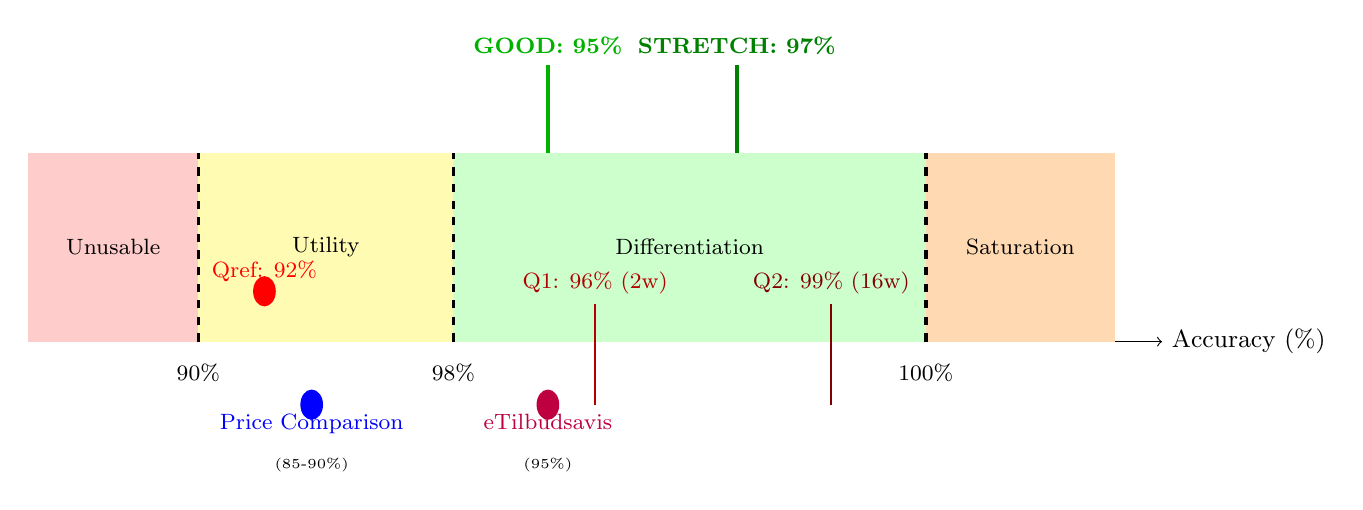
\begin{tikzpicture}[xscale=1.2, yscale=1.6]
        % Quality axis
        \draw[->] (0,0) -- (12,0) node[right] {\small Accuracy (\%)};

        % Three zones with colors
        \fill[red!20] (0,0) rectangle (1.8,1.5);
        \fill[yellow!30] (1.8,0) rectangle (4.5,1.5);
        \fill[green!20] (4.5,0) rectangle (9.5,1.5);
        \fill[orange!30] (9.5,0) rectangle (11.5,1.5);

        % Zone labels
        \node[font=\footnotesize] at (0.9,0.75) {Unusable};
        \node[font=\footnotesize] at (3.15,0.75) {Utility};
        \node[font=\footnotesize] at (7,0.75) {Differentiation};
        \node[font=\footnotesize] at (10.5,0.75) {Saturation};

        % Breakpoint lines
        \draw[very thick, dashed] (1.8,0) -- (1.8,1.5);
        \draw[very thick, dashed] (4.5,0) -- (4.5,1.5);
        \draw[very thick, dashed] (9.5,0) -- (9.5,1.5);

        % Axis labels for breakpoints
        \node[below, font=\footnotesize] at (1.8,-0.1) {90\%};
        \node[below, font=\footnotesize] at (4.5,-0.1) {98\%};
        \node[below, font=\footnotesize] at (9.5,-0.1) {100\%};

        % Competitor and product markers
        \fill[blue] (3,-0.5) circle (0.12) node[below, font=\footnotesize] {Price Comparison};
        \node[below, font=\tiny] at (3,-0.85) {(85-90\%)};
        \fill[purple] (5.5,-0.5) circle (0.12) node[below, font=\footnotesize] {eTilbudsavis};
        \node[below, font=\tiny] at (5.5,-0.85) {(95\%)};
        \fill[red] (2.5,0.4) circle (0.12) node[above, font=\footnotesize] {Qref: 92\%};

        % Cost barriers
        \draw[thick, red!70!black] (6,-0.5) -- (6,0.3);
        \node[above, font=\footnotesize, red!70!black] at (6,0.3) {Q1: 96\% (2w)};

        \draw[thick, red!50!black] (8.5,-0.5) -- (8.5,0.3);
        \node[above, font=\footnotesize, red!50!black] at (8.5,0.3) {Q2: 99\% (16w)};

        % Targets
        \draw[very thick, green!70!black] (5.5,1.5) -- (5.5,2.2);
        \node[above, font=\footnotesize\bfseries, green!70!black] at (5.5,2.2) {GOOD: 95\%};

        \draw[very thick, green!50!black] (7.5,1.5) -- (7.5,2.2);
        \node[above, font=\footnotesize\bfseries, green!50!black] at (7.5,2.2) {STRETCH: 97\%};

    \end{tikzpicture}
    \caption{QUPER Roadmap for QR1: Accuracy (Price Data Correctness)}
    \label{fig:qr1_roadmap}
\end{figure}

\textbf{Saturation Interpretation:} Beyond 98\%, each additional percentage point requires exponentially increasing effort with minimal user perceived benefit.

\subsubsection{QR5: Scalability - Concurrent User Capacity (QUPER Analysis)}

\textbf{Requirement:} The system shall support at least 300 concurrent users while maintaining acceptable performance (response time under 10 seconds), measured during peak usage hours.

\vspace{0.2cm}

\textbf{Rationale:} Scalability requires QUPER analysis because infrastructure costs increase significantly at different capacity levels, and target selection involves substantial infrastructure investment decisions.

\begin{table}[H]
\centering
\begin{tabular}{|p{14cm}|}
\hline
\textbf{FEATURE:} System Infrastructure \\
\textbf{ID:} QR5 \\
\textbf{QUALITY REQUIREMENT:} Concurrent user support \\
\hline
\textbf{DEFINITION:} The maximum number of users who can simultaneously use the application while maintaining acceptable performance (response time under 10 seconds), measured during peak usage hours. \\
\hline
\textbf{REFERENCE LEVELS} \\
\textbf{PRODUCT:} Small recipe apps \textbf{LEVEL:} 100-500 concurrent users \\
\textbf{PRODUCT:} eTilbudsavis scale \textbf{LEVEL:} 1000+ concurrent users \\
\textbf{PRODUCT:} Current CookWise \textbf{LEVEL:} N/A (new system) \\
\hline
\textbf{QUALITY BREAKPOINTS} \\
\textbf{UTILITY:} 50 concurrent users \textbf{RATIONALE:} Minimum viable capacity for initial launch in Swedish market. Below this, system cannot support even limited regional adoption and MVP launch becomes impractical. \\
\textbf{SATURATION:} 5000 concurrent users \textbf{RATIONALE:} Capacity beyond 5000 exceeds realistic projections for initial Swedish market penetration. Infrastructure investment at this scale cannot be justified for early-stage product. \\
\textbf{DIFFERENTIATION:} 500 concurrent users \textbf{RATIONALE:} Capacity of 500 supports significant market share in target regions (Karlskrona and surrounding areas) and enables positive growth trajectory. \\
\hline
\textbf{COST BARRIERS AND INFRASTRUCTURE INVESTMENT} \\
\textbf{Qref:} 100 concurrent users - Basic single-server deployment \\
\textbf{Q1:} 500 concurrent users \textbf{RATIONALE:} Load balancing, database connection pooling, query optimization, caching layer. Requires significant architecture improvements and database tuning. \textbf{Infrastructure cost implications:} Upgrading from shared hosting to dedicated server or basic cloud infrastructure (estimated additional \euro{}200-400/month operational costs). \\
\textbf{C1:} 3 weeks \\
\textbf{Q2:} 2000 concurrent users \textbf{RATIONALE:} Cloud infrastructure (AWS/Azure), CDN integration, distributed caching, auto-scaling. Requires migration to enterprise cloud platform and distributed system architecture. \textbf{Infrastructure cost implications:} Enterprise cloud tier with auto-scaling, load balancers, CDN (estimated additional \euro{}800-1500/month operational costs). \\
\textbf{C2:} 10 weeks \\
\hline
\textbf{TARGETS} \\
\textbf{GOOD:} 300 concurrent users \textbf{RATIONALE:} Realistic capacity for successful initial market launch, provides buffer for unexpected usage spikes, achievable with solid implementation and moderate infrastructure investment. \\
\textbf{STRETCH:} 500 concurrent users \textbf{RATIONALE:} Provides differentiation and growth capacity. Reaching this level requires infrastructure investment (approximately \euro{}200-400/month additional operational costs) which must be evaluated against project budget and expected user growth trajectory. \\
\hline
\textbf{VALIDATION PROCEDURE} \\
Scalability tested using load testing tools (Apache JMeter or Locust) simulating multiple concurrent users performing typical tasks (searching recipes, creating shopping lists). Tests gradually increase concurrent users until response time exceeds 10 seconds or error rate exceeds 1\%. Maximum concurrent users before performance degradation recorded. Testing conducted in staging environment mirroring production configuration. \\
\hline
\end{tabular}
\caption{QR5: Scalability Quality Requirement with QUPER Analysis}
\label{tab:qr5}
\end{table}

\textbf{Note on Infrastructure Costs:} Scaling from the Good level (300 users) to the Stretch level (500 users) involves both one time development costs and recurring monthly infrastructure expenses.

\subsubsection{QR2, QR3, QR4: Additional Quality Requirements}

The following quality requirements have straightforward targets based on industry standards and user expectations, and do not require detailed QUPER analysis:

\vspace{0.3cm}

\textbf{QR2: Reliability - System Uptime}
\begin{itemize}
    \item \textbf{Requirement:} The system shall maintain at least 98\% uptime during peak usage hours (17:00-20:00 local time).
    \item \textbf{Validation:} Uptime monitored using automated health checks every 60 seconds. Downtime incidents logged and analyzed. Monthly uptime percentage calculated as (total available minutes / total minutes in peak hours) × 100.
    \item \textbf{Rationale:} 98\% uptime is acceptable for MVP launch while maintaining user trust.
\end{itemize}

\vspace{0.3cm}

\textbf{QR3: Performance - Recipe Generation Response Time}
\begin{itemize}
    \item \textbf{Requirement:} The system shall generate recipe suggestions within 5 seconds for 95\% of user requests.
    \item \textbf{Validation:} Response times logged for all recipe suggestion requests. 95th percentile response time calculated weekly from logs. Measured from user search submission to complete result display.
    \item \textbf{Rationale:} Users expect web applications to respond within 5 seconds for satisfactory engagement.
\end{itemize}

\vspace{0.3cm}

\textbf{QR4: Usability - Time to First Recipe Selection}
\begin{itemize}
    \item \textbf{Requirement:} The system shall enable new users to complete their first recipe selection within 8 minutes of account creation.
    \item \textbf{Validation:} User session analytics track time from login to first recipe added to shopping list. Median completion time calculated monthly from new user cohorts. Users unable to complete task within 15 minutes flagged for usability investigation.
    \item \textbf{Rationale:} 8 minutes is a reasonable timeframe for new users to explore the interface and make their first selection.
\end{itemize}
